\chapter{Vergleich}
Welche Ansätze existieren bereits, um Abfragen an CSV-Dateien auszuführen? Grob lassen sich diese in zwei Kategorien unterteilen: Programme, die mit ihrer eigenen Syntax SQL-ähnliche Funktionen imitieren, und solche, die SQL-Abfragen ohne Datenbank auf Textdateien ausführen.

\section{SQL-ähnliche Syntax}
\subsection{Datamash}
Ein wunderbares Programm für die Analyse auf Textdateien ist \textit{datamash},
\footnote{\url{http://www.gnu.org/software/datamash/}}
das numerische Operationen auf Datensätze ausführen kann und dabei auch die meisten Operationen des $\gamma$-Operators beherrscht. Das Programm ist in C geschrieben, arbeitet ausschließlich als Filter für DSV-Dateien (Trennzeichen standardmäßig Tab) und erwartet in den Optionen die Spalten nach denen gruppiert wird und als Argument die auszuführende Aktion.
\begin{lstlisting}[language=Bash]
$ cat myexample
A	1
A	3
B	2
$ cat myexample | datamash sum 2
6
$ datamash -g1 sum 2
A	4
B	2
\end{lstlisting}

Um das Programm in die Skripte der TPC-H-Abfragen einzubinden, soll es Kopfzeilen erkennen und das Trennzeichen muss variabel bestimmt werden. Beides kann datamash, die Option \textit{--headers} oder \textit{-H} weist die erste Zeile als Kopf aus und mit \textit{--field-separator=,} oder \textit{-t,} wird das Komma ',' als Separator bestimmt.
\begin{lstlisting}[language=Bash]
$ cat myexample
Name,Zahlen
A,1
A,3
B,2
$ datamash -H -t, -g1  sum 2
Name,sum(Zahlen)
A,4
B,2
\end{lstlisting}

Sieht das Gruppieren und anschließende Summieren, Zählen, Mittelwertbilden kompliziert aus, so dient jetzt eine einzige Anfrage dazu, die Option \textit{-s} erspart einem sogar das vorherige Sortieren, nachfolgend die angepasste erste TPC-H Abfrage (erste Berechnung weiterhin mit awk).

\begin{lstlisting}[language=Bash]
#!/bin/bash
#2014-09-01
cat lineitem.* | awk -F\| '
        NR==1{
                print $0 "sum_disc|sum_charge|"
        }
        NR>1 && $11<="1998-9-2"{
                suma=($6*(1.0-$7));
                sumb=($6*(1.0-$7)*(1.0+$8));
                print $0 suma "|" sumb "|"
        }
' > tmp.csv
head -1 tmp.csv > tmp1.csv
tail -n+2 tmp.csv | sort -t\| -k9,10 | cat tmp1.csv - |\
datamash -t\| -H -g9,10 sum 5 sum 6 sum 17 sum 18 mean 5 mean 6 mean 7 count 1
\end{lstlisting}

Zu beachten ist, dass datamash Dezimalzahlen im länderspezifischen Format ausgibt und auch solche in der Eingabe benötigt. Sind die Datensätze auf ein anderes Format ausgelegt, so sind meist '.' und ',' ganz einfach durch den Befehl \textit{tr} zu vertauschen.
\begin{lstlisting}[language=Bash]
$ cat datei |  tr '.,' ',.'
\end{lstlisting}

Auf diese Weise werden die Skripte mit datamash geschrieben und auch wieder die Zeit gemessen.

%\begin{figure}[b]
\begin{tikzpicture}
\begin{axis}[
xtick=data,
legend style={at={(0.5,0.97)},
         anchor=north,legend columns=-1},
title=Abfragedauer bei SF1,
width=0.95\textwidth,height=0.48\textheight,
ybar = 0.25pt,
bar width=6pt,
xlabel={$Abfrage Nr.$},
ylabel={$Zeit [s]$},
]
\addplot[
ybar,
fill = blue,
] plot coordinates {
(1,47.420)
(2,6.372)
(3,32.022)
(4,22.544)
(5,26.827)
(6,7.949)
(7,18.713)
(8,39.677)
(9,54.243)
(10,12.971)
(11,2.934)
(12,22.859)
(13,7.068)
(14,7.185)
(15,29.784)
(16,4.957)
(17,37.156)
(18,25.484)
(19,6.728)
(20,58.405)
(21,63.225)
(22,6.178)
};
\addplot[
ybar,
fill  = orange
] plot coordinates{
%datamash
(1,61.962)
(2,6.494)
(3,28.086)
(4,22.332)
(5,37.344)
(6,8.024)
(7,23.258)
(8,24.036)
(9,45.607)
(10,15.708)
(11,3.037)
(12,23.359)
(13,7.992)
(14,8.099)
(15,7.581)
(16,3.532)
(17,48.223)
(18,18.802)
(19,8.611)
(20,11.221)
(21,43.384)
(22,6.565)
};
\legend{Abfragen nur mit awk, Abfragen mit datamash}
\end{axis}
\end{tikzpicture}
%\end{figure}

In den meisten Fällen sind die umgeschriebenen Skripte langsamer, in manchen aber auch deutlich schneller. Der Vorteil an den Skripten, die ausschließlich awk nutzen, ist, dass Berechnungen und das Gruppieren in einem Schritt erfolgen kann. datamash unterstützt nur Aggregatsfunktionen und keine arithmetischen Ausdrücke, sodass für Berechnungen ein weiteres Programm benötigt wird. Der Vorteil von datamash liegt aber in der Einfachheit, mit der Aggregatsfunktionen eingegeben werden können.
Auf der Seite zu datamash sind auch äquivalente Kommandos mit anderen Programmen aufgelistet.
\footnote{\url{http://www.gnu.org/software/datamash/alternatives/}}\\\\
Fazit: datamash ist ein sehr schönes Programm, das einem die Arbeit erleichtern kann, der kompliziertere Umgang mit awk kann aber zu schnelleren Abfragen führen.

\subsection{csvtool}
Das in OCaml geschriebene csvtool ist mittlerweile in allen Linux-Pa\-ket\-ver\-wal\-tungs\-sys\-te\-men erhältlich und richtet sich an Nutzer mit komplizierteren CSV-Datensätzen.
\footnote{\url{https://forge.ocamlcore.org/projects/csv/}}
Im Grunde ersetzt das csvtool die klassischen Unix-Werkeuge wie grep, cut, head, tail, join, wc -l, usw., jedoch kann es auch problemlos mit Spezialfällen hantieren, in denen sich ein Datensatz über mehrere Zeilen erstreckt.
Die Selektion heißt dort \textit{namedcol}.
\begin{lstlisting}[language=Bash]
$ csvtool namedcol ID,Name Punktetabelle.csv 
1,Franz
2,Alfred
3,Marie
\end{lstlisting}

Für Joins ist csvtool nur bedingt geeignet, die Syntax ist alles andere als intuitiv.
\begin{lstlisting}[language=Bash]
$ csvtool join <Joinattribute> <Tabellennummer> Tabelle1 Tabelle2
\end{lstlisting}

Bei Joinattribute werden beginnend bei 0 die zu vergleichenden Spalten eingetragen, bei Tabellennummer als Liste die Spalten, die später sichtbar sein sollen. Dabei bezieht sich die Auswahl aber immer auf beide Tabellen, folglich müssen Joinattribute an der gleichen Position stehen.

\begin{lstlisting}[language=Bash]
$ csvtool join 1 2,3 Punktetabelle.csv Zeittabelle.csv 
1,Franz,50,44,
2,Alfred,10,88,
3,Marie,27,67,
ID,Name,Punkte,Zeit,
\end{lstlisting}

Für relationale Algebra ist das Programm weniger gedacht als für einfach Vergleiche von CSV-Datensätzen. Für komplizierte Abfragen empfehlen sich mächtigere Programme, die in den meisten Fällen auch SQL-Ausdrücke beherrschen und deshalb noch vorgestellt werden.

\subsection{Fsdb}
Seit 1991 existiert Fsdb als eine textdateibasierte Datenbank (flat text database for shell scripting), die jedoch ihrem eigenen Datenformat gehorcht und Operationen ähnlich zu datamash beherrscht.
\footnote{\url{http://www.isi.edu/~johnh/SOFTWARE/FSDB/}}

Die Textdateien enden auf \textit{.fsdb}, am Anfang steht eine Kopfzeile, gekennzeichnet durch "'\#fsdb"', mit den Spaltenbezeichnern, anschließend die durch Leerräume separierten Werte.
Das Feldtrennzeichen kann mit \textit{-F} verändert werden, Kommentare beginnen mit '\#', mit dem Befehl \textbf{csv\_to\_db} können CSV-Dateien in das Format konvertiert werden.

\begin{lstlisting}
$ cat Punktetabelle.fsdb
#ID Name Punkte
1 Franz 50
2 Alfred 10
3 Marie 27
$ cat Punktetabelle.fsdb | dbcol ID Name Punkte
#fsdb ID Name Punkte
1	Franz	50
2	Alfred	10
3	Marie	27
\end{lstlisting}

Die Kommandos von Fsdb arbeiten als Filter, sie lesen also von der Standardeingabe Daten ein, die immer im entsprechenden Format stehen müssen. Insgesamt eine nette Idee, das Erlernen der vielen verschiedenen Kommandos nur eher unintuitiv.

\section{Abfragen mit SQL}

\begin{figure}
\centering
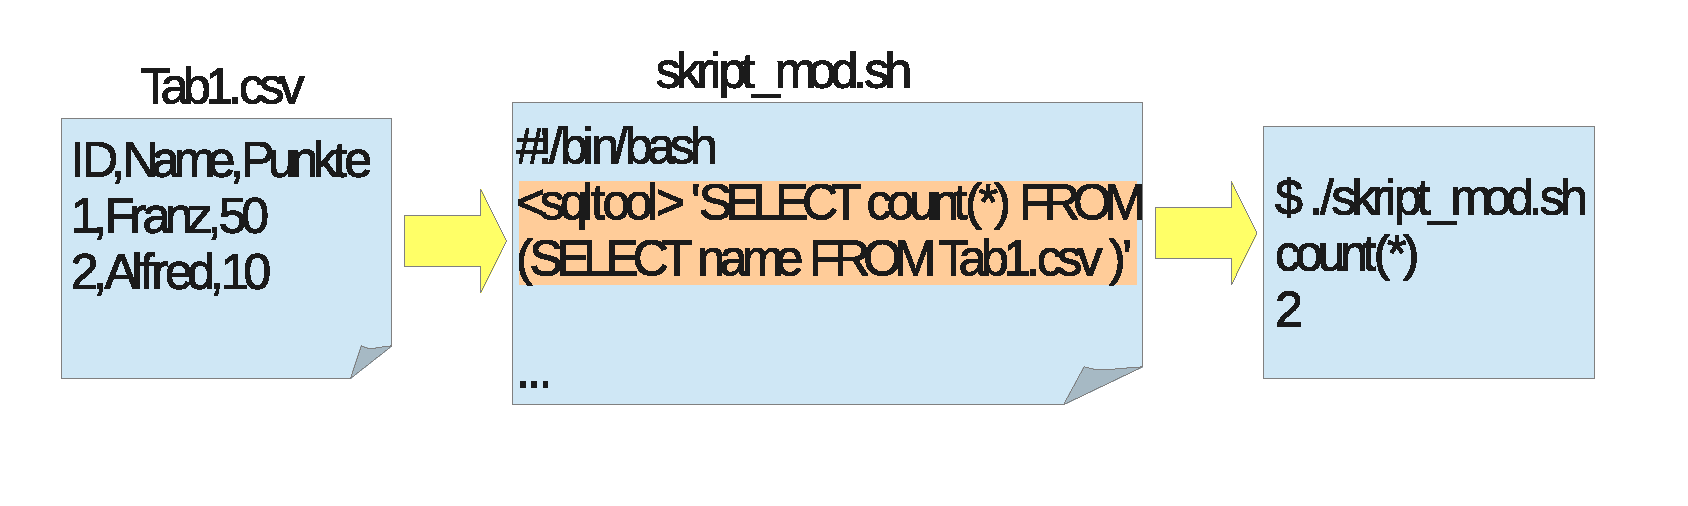
\includegraphics[scale=.4]{vergleich.eps}
\caption{Funktionsweise von SQL-Tools in der Kommandozeile}
\label{fig:vergleich}
\end{figure}

\subsection{txt-sushi}
Ein geniale Sammlung von Programmen, um auf CSV-Dateien mit SQL-Syntax zuzugreifen ist \textbf{txt-sushi}. Einmal installiert, so bietet es neben zahlreichen weiteren Funktionen, die die Ausgabe von Textdateien verschönern, auch ein Programm \textbf{tssql} an, mit dem sich in SQL formulierte Abfragen auf CSV-Dateien ausführen lassen.
\footnote{\url{http://keithsheppard.name/txt-sushi/}}

\begin{lstlisting}[language=Bash]
$ tssql 'select * from `orders.csv`'
O_Id,OrderDate,OrderPrice,Customer
1,2008/11/12,1000,Hansen
2,2008/10/23,1600,Nilsen
3,2008/09/02,700,Hansen
4,2008/09/03,300,Hansen
5,2008/08/30,2000,Jensen
6,2008/10/04,100,Nilsen
\end{lstlisting}
Das Programm arbeitet auch als Filter und kann von der Standardausgabe lesen, die Daten können über eine Pipe weitergereicht werden. Generell gilt, alle Daten, die eingelesen werden sollen, werden mit zwei Gravis (back tick, ' ` ') geklammert.
\begin{lstlisting}[language=Bash]
$ cat orders.csv | tssql 'select * from `-`'
O_Id,OrderDate,OrderPrice,Customer
1,2008/11/12,1000,Hansen
2,2008/10/23,1600,Nilsen
...
\end{lstlisting}

Noch einfacher können die Tabellen gleich über Optionen eingebunden werden, dort werden auch Bezeichner für die Dateien definiert.
\begin{lstlisting}[language=Bash]
$ tssql -table orders orders.csv 'select * from orders'
\end{lstlisting}

Leider akzeptiert das Programm nur durch Komma separierte Dateien, wird ein anderes Symbol als Trennzeichen verwendet, so muss das über eine Umlenkung erfolgen.
\begin{lstlisting}[language=Bash]
$ tssql -table orders <(sed 's/;/,/g' orders_mit_Semikolon.csv) 'select * from orders'
\end{lstlisting}
Probleme bereitet dies, wenn Kommata Bestandteil der Datensätze sind. Am einfachsten ist es, den Programmcode so umzuschreiben, sodass ein anderes Zeichen die Daten voneinander trennt. (Die Quelldateien finden sich auf Github, zu verändern ist die Datei \textit{txt-sushi-master/Database/TxtSushi/FlatFile.hs})
\footnote{\url{https://github.com/keithshep/txt-sushi}}

So kann auch ein einfaches Skript geschrieben werden, um größere SQL-Abfragen gemäß dem TPC-H Schema einzugeben.
\begin{lstlisting}[language=Bash]
#!/bin/bash
TSSQL=/home/maximilian/Downloads/txt-sushi-master/tssql
$TSSQL -table lineitem <(cat lineitem.*) '
SELECT
        l_returnflag,
        l_linestatus
FROM
        lineitem
GROUP BY
        l_returnflag,
        l_linestatus
'

\end{lstlisting}
Bei der Ausführung selbst einfacher Abfragen wie der gerade beschriebenen stellt man schnell fest, dass der Arbeitsspeicher den limitierenden Faktor darstellt. Sobald größere Operationen durchgeführt werden, die über eine Selektion hinausgehen, so lädt das Haskell-Programm alle Datensätze in den Hauptspeicher. Das beschriebene Skript wird nach einiger Zeit durch das System beendet. Für große Datenmengen ist das Programm nicht geeignet, obwohl es in der Bedienung und von der Funktion einzigartig gut und praktisch ist.

\subsection{csvfix}
Die meisten Datenbanksysteme unterstützen den Import von CSV-Dateien, aber leider nicht alle. Besonders im mobilen Bereich, wo Anwender auf gewisse Datenbanken nur über eine SQL-Schnittstelle zugreifen können, sind SQL-Anweisungen zum Einfügen von Daten von Vorteil (s. Abb. \ref{fig:konvert}). Dagegen hilft csvfix, das aus gegebenen CSV-Datensätze entsprechend viele INSERT-/UPDATE/- oder DELETE-Anweisungen generiert. Einfach den Tabellennamen, die Spaltenbezeichner und die Quelldatei angeben, schon werden die SQL-Anweisungen erzeugt, mit der Option \textit{-ifn} wird die erste Zeile als Kopfzeile betrachtet.
\begin{lstlisting}[language=Bash]
$ cat Punktetabelle.csv
ID,Name,Punkte
1,Franz,50
2,Alfred,10
3,Marie,27
$ csvfix sql_insert -ifn -t punktetabelle -f 1:ID,2:Name,3:Punkte Punktetabelle.csv
INSERT INTO punktetabelle ( ID, Name, Punkte ) VALUES( '1', 'Franz', '50');
INSERT INTO punktetabelle ( ID, Name, Punkte ) VALUES( '2', 'Alfred', '10');
INSERT INTO punktetabelle ( ID, Name, Punkte ) VALUES( '3', 'Marie', '27');
\end{lstlisting}

Über die Option \textit{-sep} kann noch das Feldtrennzeichen angegeben werden, sollen Felder ohne Anführungszeichen ausgegeben werden, so dient die Option \textit{-nq} dazu.
\begin{lstlisting}[language=Bash]
$ csvfix sql_insert -ifn -sep , -t punktetabelle -nq 1,3 -f 1:ID,2:Name,3:Punkte Punktetabelle.csv
INSERT INTO punktetabelle ( ID, Name, Punkte ) VALUES( 1, 'Franz', 50);
INSERT INTO punktetabelle ( ID, Name, Punkte ) VALUES( 2, 'Alfred', 10);
INSERT INTO punktetabelle ( ID, Name, Punkte ) VALUES( 3, 'Marie', 27);
\end{lstlisting}

\begin{figure}
\centering
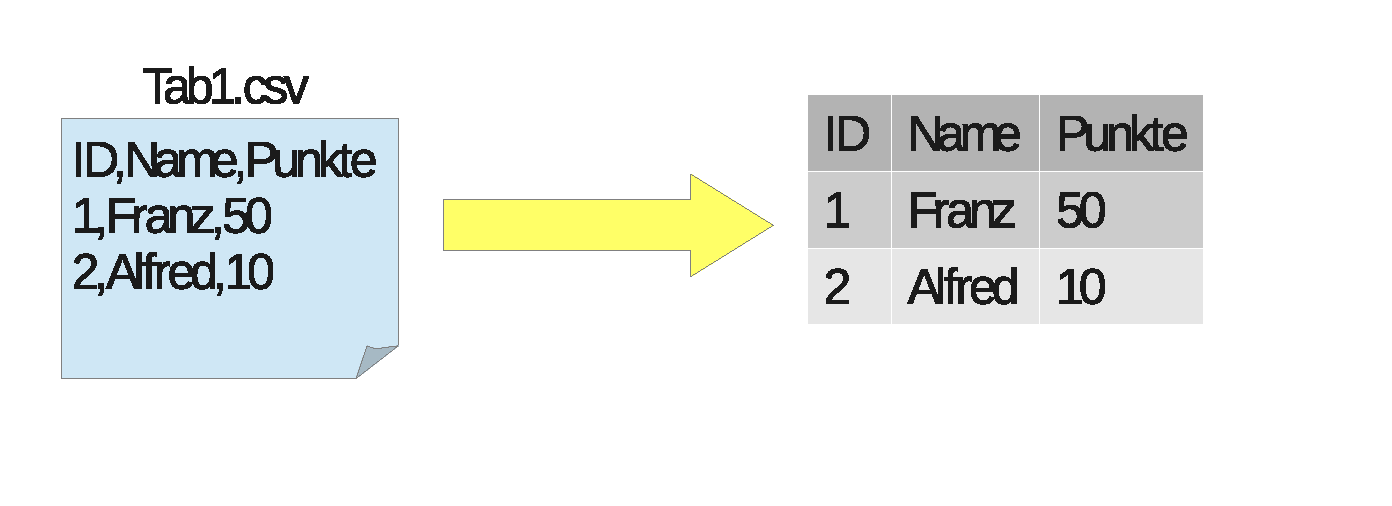
\includegraphics[scale=0.4]{konvert.eps}
\caption{Import von CSV}
\label{fig:konvert}
\end{figure}

Doch csvfix kann mehr, als nur SQL-Befehle generieren, ähnlich dem csvtool unterstützt es auch den Verbund mehrerer Tabellen und weitere arithmetische Operationen ähnlich zu awk.
\footnote{\url{http://csvfix.byethost5.com/csvfix15/csvfix.html}}
\begin{lstlisting}[language=Bash]
$ csvfix join -f 1:1 Zeittabelle.csv Punktetabelle.csv 
"ID","Zeit","Name","Punkte"
"1","44","Franz","50"
"2","88","Alfred","10"
"3","67","Marie","27"
\end{lstlisting}
Äquivalenzen werden durch den Doppelpunkt beschrieben (\textit{Feld von i : Feld von i+1}), in einem Schritt können mehrere Joins vollzogen werden, es werden einfach mehrere Quelldateien angegeben.

Generell gibt es für die meisten benötigten Kommandos ein Äquivalent in csvfix, der Vorteil liegt an den unterstützten Standards, ein Komma als Feldinhalt stellt kein Problem dar. Abgesehen von diesen Spezialfällen reichen auch die klassischen Kommandos aus.

\subsection{csvkit}
Die Funktionen von csvfix und txt-sushi kombiniert bietet das von der Literatur gepriesene csvkit \cite{DataScience}. Es unterstützt zwar auch einfache Operationen um CSV-Dateien auszugeben, ist aber primär auf das Anwenden von SQL-Abfragen auf CSV-Dateien ausgelegt und bietet an, bei größeren Datenmengen die Abfrage über eine Datenbankverbindung auszuführen.
\footnote{\url{https://csvkit.readthedocs.org/en/latest/index.html}}

Zuerst einmal ist es fähig, eine Anweisung zum Erstellen von Datenbank-Schemata auszugeben und erkennt dabei selbständig den Typ. Über die Option \textit{-i} ist die Anweisung sogar auf bestimmte Datenbanktypen zugeschnitten.
\begin{lstlisting}[language=Bash]
$ csvsql -i postgresql Punktetabelle.csv
CREATE TABLE "Punktetabelle" (
	"ID" INTEGER NOT NULL, 
	"Name" VARCHAR(6) NOT NULL, 
	"Punkte" INTEGER NOT NULL
);
\end{lstlisting}

Leider kann das Programm keine Operationen zum Einfügen direkt generieren, dafür dient csvfix. Stattdessen ist es möglich, über eine Datenbankanbindung direkt die CSV-Dateien zu importieren.

\begin{lstlisting}[language=Bash]
$ csvsql --db <Verbindung zur Datenbank> --insert Punktetabelle.csv
\end{lstlisting}

Aber nun folgt die Option \textit{--query}, um eine SQL-Anweisung direkt auszuführen, mit \textit{-d} kann auch das Trennzeichen bestimmt werden.

\begin{lstlisting}[language=Bash]
$ csvsql -d, --query 'select * from Punktetabelle' Punktetabelle.csv
ID,Name,Punkte
1,Franz,50
2,Alfred,10
3,Marie,27
\end{lstlisting}

Das Programm arbeitet nur auf CSV-Dateien, die auch eine Kopfzeile besitzen und auf die Dateiendung \textit{.csv} hören, alles andere akzeptiert es nicht, trotz Modifikation können die TPC-H Abfragen aufgrund ihrer Größe nicht ausgeführt werden.

\subsection{querycsv.py}
Das in Python geschriebene Skript querycsv.py arbeitet ähnlich und ist flexibler in der Annahme von Dateinamen.
\footnote{\url{https://pypi.python.org/pypi/querycsv}}

\begin{lstlisting}[language=Bash]
$ alias querycsv='/home/maximilian/Downloads/querycsv-0.3.0.0/querycsv/querycsv.py'
$ querycsv -i Punktetabelle.csv 'Select * From Punktetabelle'
 ID | Name   | Punkte
======================
 1  | Franz  | 50    
 2  | Alfred | 10    
 3  | Marie  | 27  
\end{lstlisting}

Dank eines CSV-Sniffers erkennt das Programm automatisch das Feldtrennzeichen, leider sind die möglichen Trennzeichen dadurch auch beschränkt, eine Pipe '|' zum Trennen wird nicht unterstützt. Ohne Modifikation der CSV-Dateien ist auch dieses Programm für die TPC-H Abfragen nicht zu nutzen.
\begin{lstlisting}[language=Python]
dialect = csv.Sniffer().sniff(open(infilename, "rt").readline())
\end{lstlisting}
Die Endung der Dateien auf \textit{.tbl} erkennt das Skript mühelos, der Name zuvor wird als Tabellenbezeichner verwendet, nur werden keine Daten ohne Kopfzeile akzeptiert, wie auch durch Pipe getrennte Dateien. Liegen die Daten der TPC-H Anfragen in einer Datei, so ist diese zu groß für das Programm. Fazit: Ein sehr schönes Skript, aber Mangel an Flexibilität.

\subsection{gcsvsql}
Ein ähnliches Programm wie csvsql, heißt gcsvsql, da es auf Groovy basiert, einer objektorientierten Skriptsprache und der Name csvsql schon vergeben ist.
\footnote{\url{https://code.google.com/p/gcsvsql/}}
Die Abfrage wird einfach als SQL-Anweisung eingegeben, als Tabelle steht der Name der CSV-Datei.
\begin{lstlisting}[language=Bash]
$ gcsvsql "select * from Punktetabelle.csv"
\end{lstlisting}

Wegen der starren Syntax und einer seltenen Programmiersprache erweist sich die Anwendung des Programms als schwierig.

\subsection{Mynodbcsv}
Einen ähnlichen Ansatz wie txt-sushi nur noch optimierter und einen Schritt weiter geht das Konzept Mynodbcsv, das vor Kurzem veröffentlicht worden ist.
Insgesamt geht es um das Problem, wie sehr große Datenmengen aus CSV-Dateien mit SQL-Anweisungen abgefragt werden, ohne dabei die kompletten Daten in eine Datenbank zu importieren und auch kein Datenbankschema vorher konfigurieren zu müssen.\\
Das Konzept analysiert anhand einer optimierten Abfrage zuerst die relevanten Felder einer CSV-Datei, anschließend lädt es nur die relevanten Daten in eine SQLite-Datenbank, worauf die Abfrage laufen kann. Somit geht dieses Konzept einen Mittelweg, es müssen nie alle Daten in eine Datenbank importiert werden, trotzdem erfolgt die Abfrage mittels eines Datenbanksystems. Für die genauen Messergebnisse sei auf die Veröffentlichung verwiesen \cite{Mynodbcsv}.

\subsection{shql}
Ähnlich der geschriebenen Abfragen als TPC-H Skripte implementiert shql eine Datenbank, die ausschließlich auf den Unix-Kommandos basiert und SQL über awk-Funktionen interpretiert.
\footnote{\url{http://lorance.freeshell.org/shql/}}
